\section{Sprint 5 - Summary}

At the beginning of sprint 5, we received the second batch of variable pitch mechanisms. These mechanisms were ordered from Rcecho.com and looked different in the picture than the first batch. Our gamble was that the first batch was fake and that the second batch were of better quality.
The mechanisms were identical to the first batch and had just as poor quality, all shafts were bent and did not function properly. It is the inner shaft in the mechanism which is bent, it could be changed, but 1,46 mm hardened steel rods are hard to come by. \\ 
\\ 
Because of the challenges with the mechanisms ordered from RCecho, new research was required. It turned out that mechanisms we initially intended to use, but not found online, were sold by a RC enthusiast in Son, Norway. We got eight of the Axi 2208 EVP units (Fig. \ref{fig:evp}) and two variable pitch ready motors: Axi 2208/26 EVP (Fig. \ref{fig:aximotor}) with hollow shafts. Two additional motors were ordered from Steve Webb Models in the UK. \\
\begin{figure}[h]
        \centering
         \begin{minipage}[b]{0.4\textwidth}
            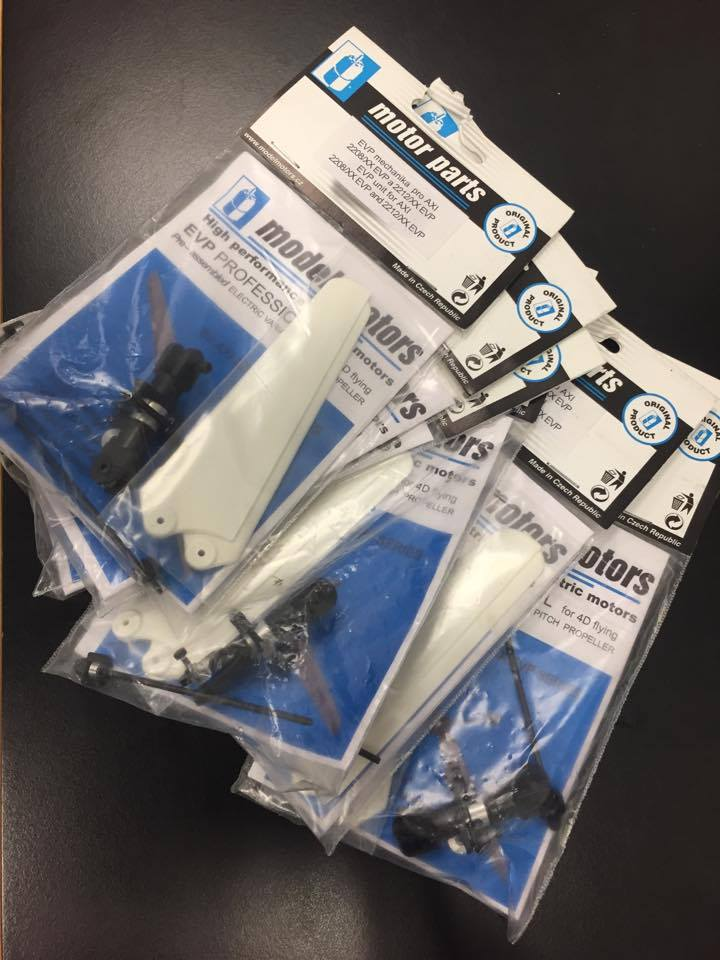
\includegraphics[width = 1\textwidth]{VAPIQ-PICTURES/axievp}
              \caption{Axi Electric Variable Pitch Unit}
            \label{fig:evp}
        \end{minipage}
        \hfill
        \begin{minipage}[b]{0.4\textwidth}
            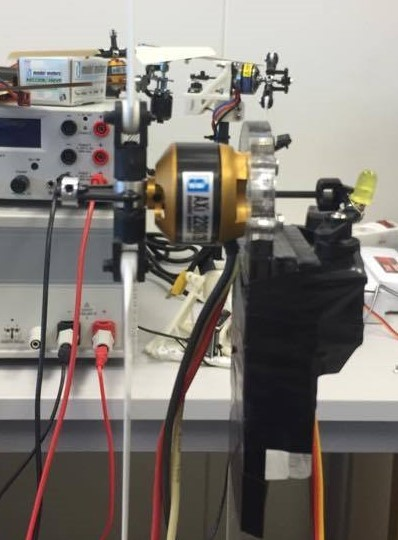
\includegraphics[width = 1\textwidth]{VAPIQ-PICTURES/axi2208}
            \caption{Axi 2208/26 EVP Motor}
            \label{fig:aximotor}
        \end{minipage}
\end{figure}

The group has made improvements in the flight controller code. After running tests, we discovered that it works well until we mount the propellers, which introduces vibrations. 
 
When the vibrations get high, the IMU gives very unstable data. We must continue the sprint to research how to filter the sensor data, and reduce the noise. To mechanically reduce vibrations, rubber gaskets have been mounted under the motors and the IMU has been placed in vibration dampening material.

\subsection{Completion and Scope Change}

\subsection{Results and Conclusions}

%prosjektplan
\begin{comment}


Sprint 5:
Scrum Ceremonies
Manually Scheduled	Mechanical Design Review 
Mechanical Improvements
Flight Testing And Control
Servo Control, Variable Pitch
Controller
Advanced Control Functionallity 
Acceptance Testing


Ting å få med:

-V-pitch Rig
-Noise!!!! Noise!!
-Mechanisms did not work-> new plan
-New machanisms from deep in the basment of rc dude in Son0


  \begin{itemize}
        \item Prototype, Variabel Pitch, \textbf{Done} (Mechanisms produced to little thrust and quadcopter was to heavy)
        \item Matlab and Simulink Simulation, \textbf{Postponed}
        \item Stabilization And Regulation, \textbf{In progress}
        \item Tweak Flight Controller, Fixed Pitch, \textbf{In progress}
    \end{itemize}



\end{comment}